%%%--------------------------------%%%
%%% UC9
%%%--------------------------------%%%

\newpage
% UC9 ====================================================
\subsubsection{Use Case Specification: \ac{UC}9 Project Initialization}
\label{sec:domainBbj}

\paragraph*{Description}\mbox{}\\
To begin with the risk management process inital risk contributions are needed. Therefore a project is initialized with a starting challenge. The project manager sets an initial number of risks to be contributed, a deadline for them and a minimum number of supporters for a risk to be accepted into the discussion, as well as a deadline for the initial discussion process.

\paragraph*{Screenshots}\mbox{}\\
Insert screenshots and shortly explain what can be seen
\begin{figure}[h] 
	\centering
	
\includegraphics[width=0.1\textwidth]{Content/Domain/placeholder.png}
	\caption{Use Case X: Detail}
	\label{fig:label9}
\end{figure}

\paragraph*{Basic Flow} \mbox{}\\

\begin{itemize}
	\vspace{-3mm}
	\setlength\itemsep{-1em}
	\item The project manager opens an unitialized project.
	\item They enter the above described paramters.
	\item They press the initialize button.
	\item All project members are notified.
\end{itemize} 

\subparagraph{Activity Diagram}\mbox{}\\
\begin{figure}[H]
	\centering
	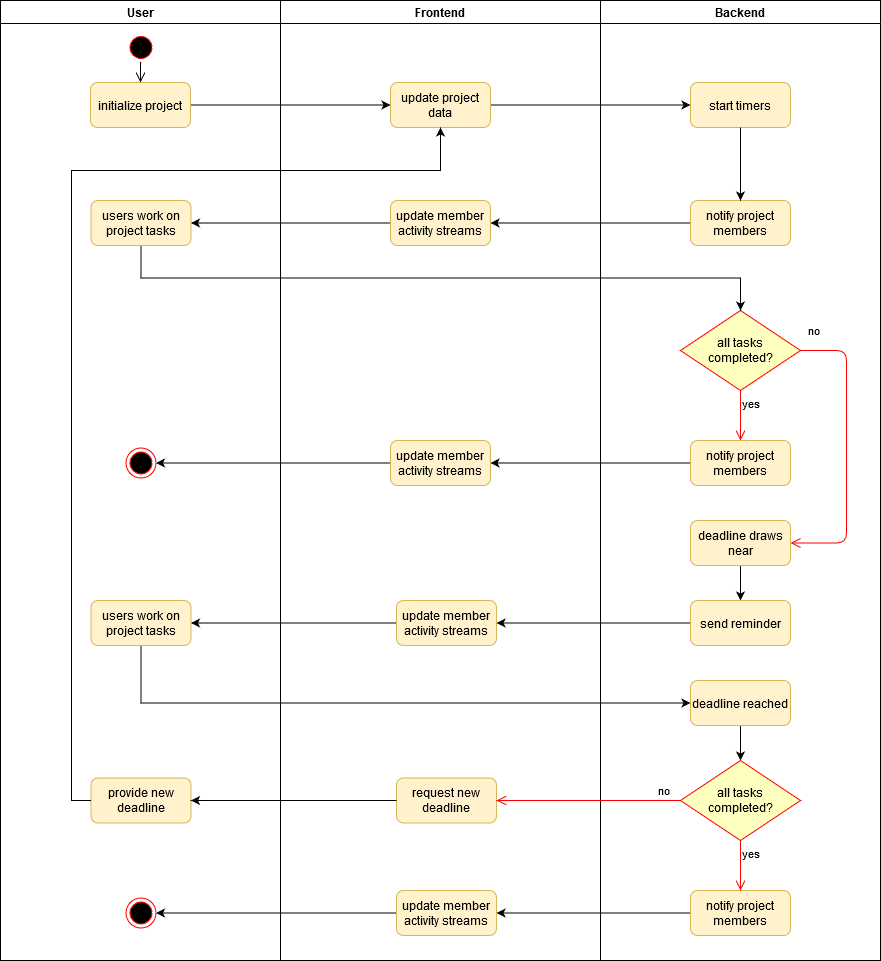
\includegraphics[width=1.0\textwidth]{Content/Domain/UC9Initialization.png}
	\caption{Activity Diagram  \ac{UC}9 Project Initialization}
	\label{fig:label14}
\end{figure}

\paragraph*{Alternative Flows}\mbox{}\\
The initalization is canceled.

\paragraph*{Special Requirements and Preconditions}\mbox{}\\
\begin{enumerate}
	\vspace{-3mm}
	\setlength\itemsep{-1em}
	\item The user is a project manager.
	\item The project manager has already created a new project.
\end{enumerate}

\paragraph*{Postconditions and Persistance}\mbox{}\\
The project will only be accessible and contain all its other described functions after being initialized.


